Ein Vergleich der in dieser Arbeit angeführten Systeme \textbf{Pastry} und
\textbf{Tapestry} bzw. artverwandter Systeme liefert untenstehende Tabelle \cite{HildrumKRZ02}.
\\
\begin{table}[H]
\begin{tabular}{|l|c|c|c|c|}
\hline
\textsc{System} & \textsc{Insert Cost} & \textsc{Space per Node} & \textsc{Hops}
& \textsc{Balance}\\ \hline
\hline
CAN & $O(d n^{1/d})$ & $O(d)$ & $O(d n^{1/d})$ & ja\\
CAN, $d = \log n$ & $O(\log n)$ & $O(\log n)$ & $O(\log n)$ & ja\\
Chord & $O(\log^2 n)$ & $O(\log n)$ & $O(\log n)$ & ja\\
\textbf{Pastry} & $O(\log^2 n)$ & $O(\log n)$ & $O(\log n)$ & ja\\
\textbf{Tapestry} & $O(\log^2 n)$ & $O(\log n)$ & $O(\log n)$ & ja\\
\hline
\end{tabular}
\end{table}
Die Grafik aus Abbildung \ref{fig:performance} zeigt den Aufwand beim Routing
für beide Systeme, Pastry und Tapestry.
\begin{figure}
  \centering 
  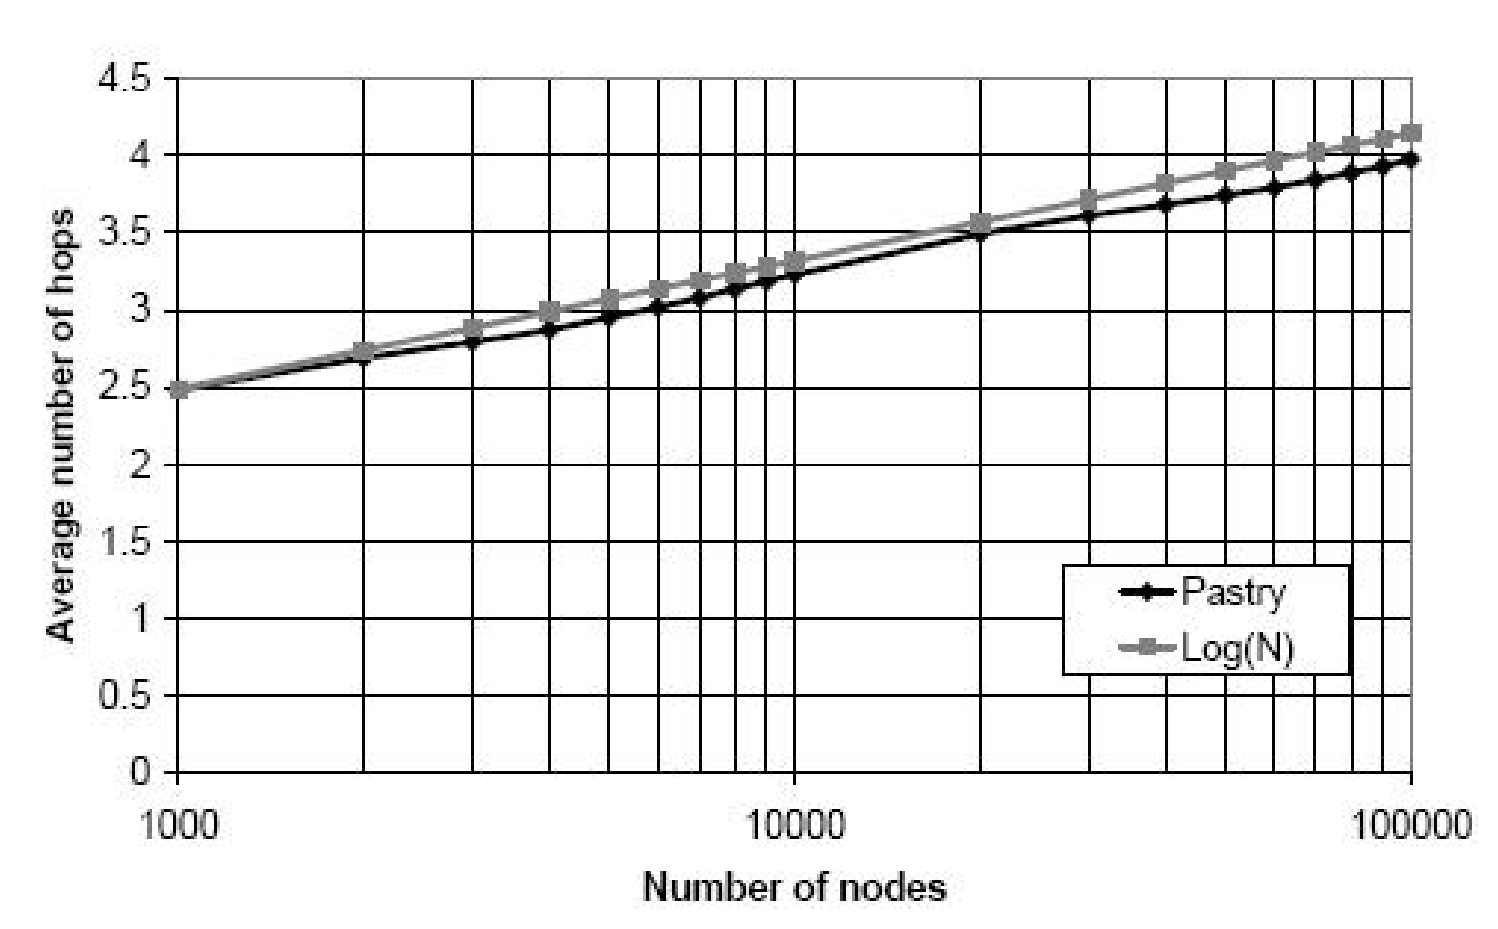
\includegraphics[width=0.8\textwidth]{../images/performance}
  \caption[Pastry und Tapestry: Performance]Routing-Performance bei Pastry und Tapestry \cite{Pastry-Middleware}
  \label{fig:performance}
\end{figure}
Die im Rahmen dieser Ausarbeitung vorgestellten Algorithmen ermöglichen die
Lokalisierung eines Objekts in logarithmischer Zeit zur Anzahl der Knoten
innerhalb eines Netzwerks.
